\begin{figure}[!htb]
\centering

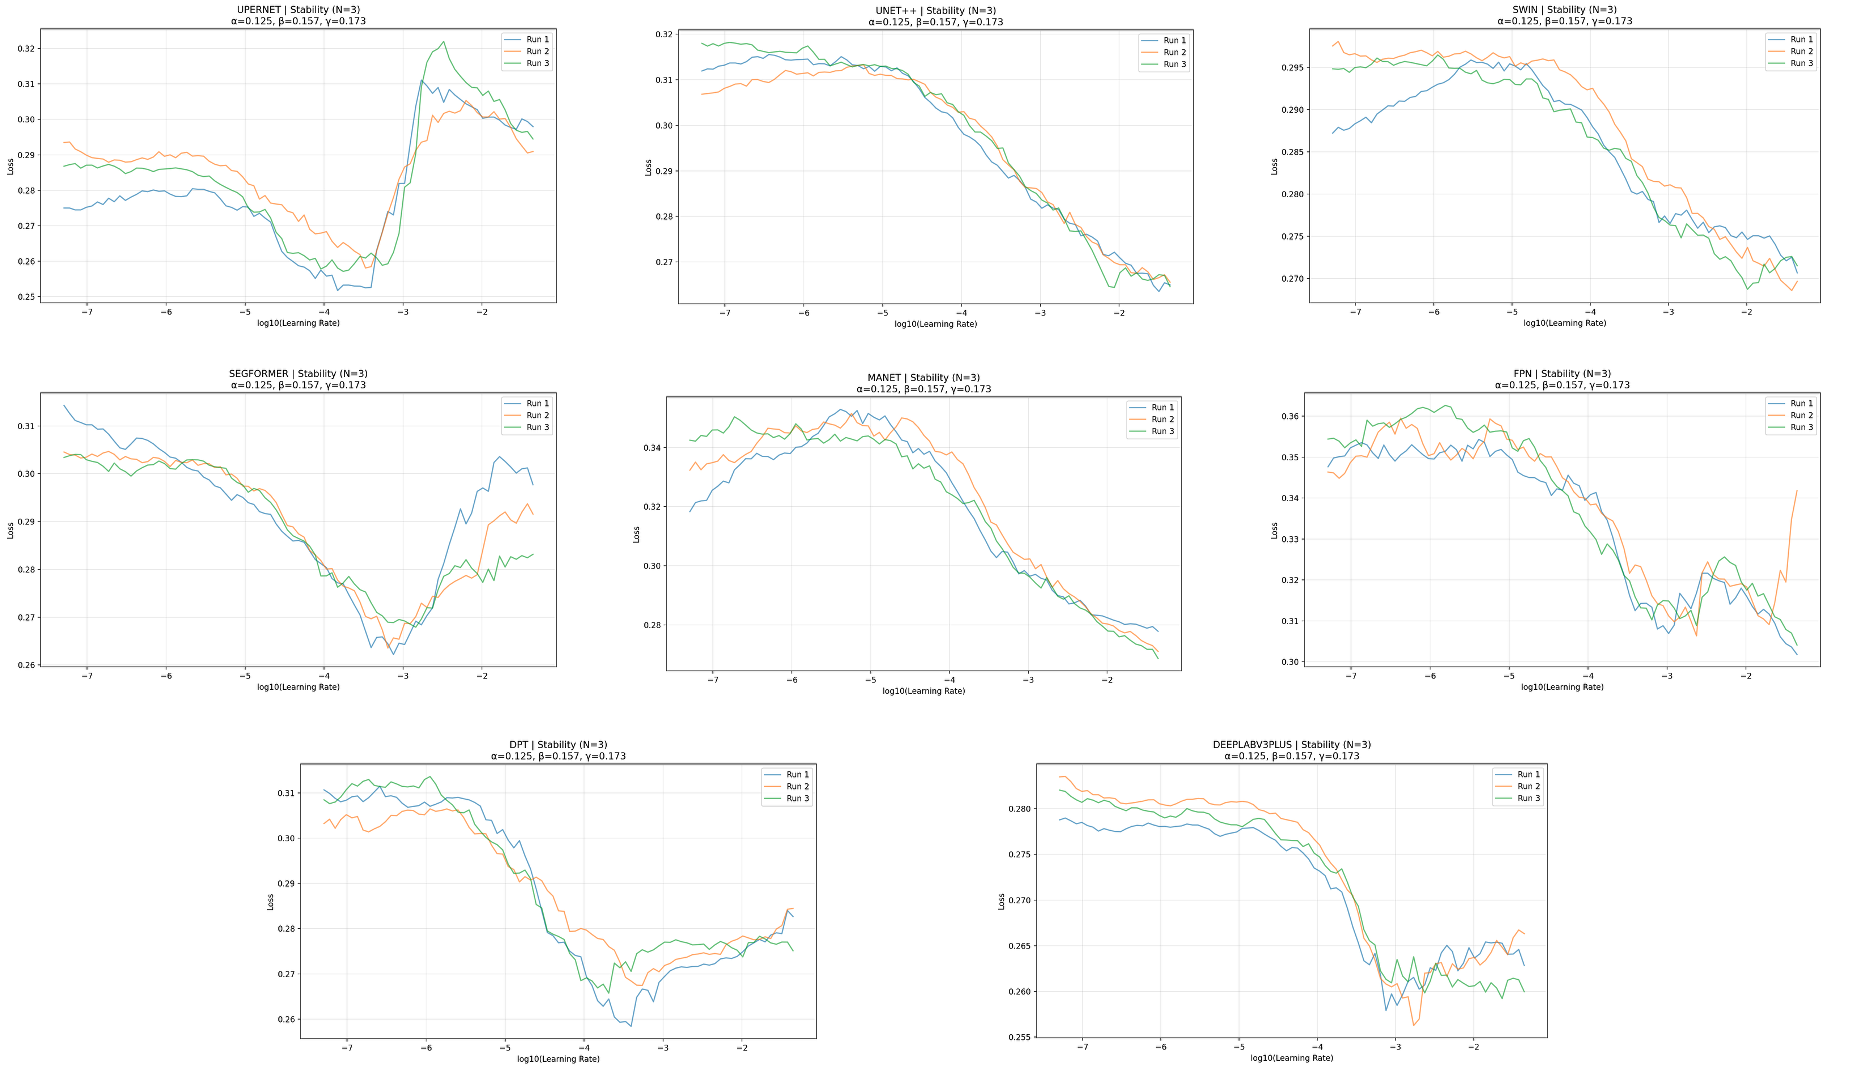
\includegraphics[width=\textwidth]{figuras/DIAGSET_MACENKO_LR.png}

\caption[Curvas de busca de taxa de aprendizado para DIAGSET com Macenko]{
Curvas de busca de taxa de aprendizado para os modelos treinados no conjunto
DIAGSET com normalização de cor pelo método de Macenko. Cada subgráfico deverá
apresentar a evolução da função de perda em função de $\log_{10}$ da taxa de
aprendizado para uma arquitetura avaliada, preferencialmente com múltiplas
execuções independentes. As curvas são utilizadas para identificar regiões de
queda estável da perda e selecionar taxas de aprendizado candidatas para o
treinamento final.
}
\label{fig:results_diagset-lr-curves-macenko}
\end{figure}

\begin{table}[!htb]
\centering
\caption{Taxas de aprendizado selecionadas para o treinamento final no DIAGSET com normalização Macenko.}
\label{tab:results_diagset-learning-rates-macenko}
\begin{tabular}{lr}
\toprule
Arquitetura & LR ($10^{-3}$) \\
\midrule
DEEPLABV3PLUS & 0.1 \\
DPT & 0.1 \\
FPN & 0.1 \\
MANET & 3.0 \\
SEGFORMER & 0.1 \\
SWIN & 1.0 \\
UNET++ & 3.0 \\
UPERNET & 0.03 \\
\bottomrule
\end{tabular}
\end{table}
